\section{Test}\label{sec:s4test}
% metatext
In this section the performed full system test will be documented.
The test is an acceptance test, and is performed to verify that the solution complies with the established requirement specification.
The acceptance test will be designed to test the whole system with some manually generated data.
The scope of the test is to check that the 'Must-have' requirements from Section \ref{sec:req} are fulfilled.
Some requirements are validated as working in previous tests, and these are omitted from the acceptance test. 
First the test design is explained and described and, subsequently, the test execution and results are documented.

% paragraph listing all requirements...
The 'Must have' requirements from Section \ref{sec:req} are as follow, firstly the functional; A Graphical user interface, User accounts including login and registration, Communication with the \gls{astep} system, User location tracking and storage, Automatically determine regular routes, Automatic suggest ride sharing partners. The two nonfunctional requirements are; Development cooperation with the other \gls{astep} project groups and User privacy.

% previously tested requirements
There have been extensive tests of the solution parts during the development, and the test results fulfilling requirements do not have to be performed again.
'User location tracking and storage', as well as 'automatic determining regular routes' were assessed acceptable in respectively Section \ref{subsec:bgstest2} and \ref{subsec:algotest}.
The latter is also partially accounting for the requirement 'suggesting ride partners' the only thing missing for this requirement, is to check whether the ride suggestions are displayed correctly to the user in the app. 
The nonfunctional requirement of development cooperation is accounted for in Section \ref{sec:grouprole}. 
The remaining requirements that needs to be accounted for and acceptance tested are the following:
\begin{itemize}
	\item Graphical user interface
	\item User accounts, including login and registration
	\item Communication with the \gls{astep} system
	\item Showing users their ridesharing matches in the app
	\item User privacy
\end{itemize}

\subsection{Acceptance Test Design}
This section is documenting the acceptance test design, and serves to describe the test method performed on the solution to evaluate the compliance with the requirements.

\todo{describe what the data is and why it's there}
Mock test data is added to the \gls{rs} server's database. 
The content can be seen in Appendix \ref{app:datadump}. 
The data sets are a combination of data pulled form the \gls{astep} database as well as data we constructed to generate matches for the test user \texttt{test}.
As we are using specialized mock data for the purpose of testing, only the user \texttt{test} has any matches.
The setup will consist of a computer running an instance of the \gls{rs} server and an android emulator.
An android emulator is used in the testing instead of an actual device so that we can avoid opening ports to the \gls{rs} server.

The first task in the test consist of opening the app and registering a new user with username \texttt{test} and the password \texttt{test}.
If this succeeds, the user is then logged out and then logged in with the same credentials.
When the user is logged into the app again, the appropriate matches stored in the \gls{rs} database will be fetched from the server and should be displayed in the app.
If the lists are shown for the user \texttt{test}, but not for the newly registered user, the overall test is completed. 

The GUI will have been tested through availability of the different functions in the app.
The user functionality will be tested when registering an user and logging in, this will also partially test the communication with the \gls{astep} system.


The rest of the requirements pertaining communication with \gls{astep} were verified in the tests performed in the previous sprints.
If the matches are pulled correctly from the \gls{rs} server and showed to the user, will be tested when the user \texttt{test} are logged in.
The requirement concerning user privacy is tested be seeing if location data about other users are displayed to the user currently logged in. 


\subsection{Performing the Test}
First a new user, \texttt{user22} was created as can be seen in Figure \ref{s4tp:newuser}.
In the process of creating a new user, some unexpected behavior regarding Scandinavian letters were observed.
Some additional tests were performed to further explore this observation, and they can be seen in Table \ref{tab:logintest}.
\begin{table}[!ht]
	\centering
	\begin{tabular}{@{}lll@{}}
		Username & Password & Result \\
		\hline
		a & a & 200 OK\\
		ø & ø & 404 not found\\
		å & a & 404 not found\\
		b & å & 401 unauthorized\\
	\end{tabular}
	\caption{Registered users login test.}
	\label{tab:logintest}
\end{table}

Some additional \gls{astep} API test leads us to believe that this is an problem in the Android application as the special characters is working correctly when tested directly in the \gls{astep} API web interface.

The registering of the user \texttt{user22} was later successfully executed when using standard English letters and can be seen in the right side of Figure \ref{s4tp:numain}. 
As expected, no matches were found to the newly registered user \texttt{user22}. 
The user was then logged out of the app.
The user \texttt{test} was then, as seen in Figure \ref{s4tp:logintest}, logged in successfully, and redirected to the main interface of the app, where the user was presented with the appropriate matches, shown in \ref{s4tp:testmain}.

\begin{figure}[ht!]
\centering
\begin{subfigure}[b]{0.24\textwidth}
        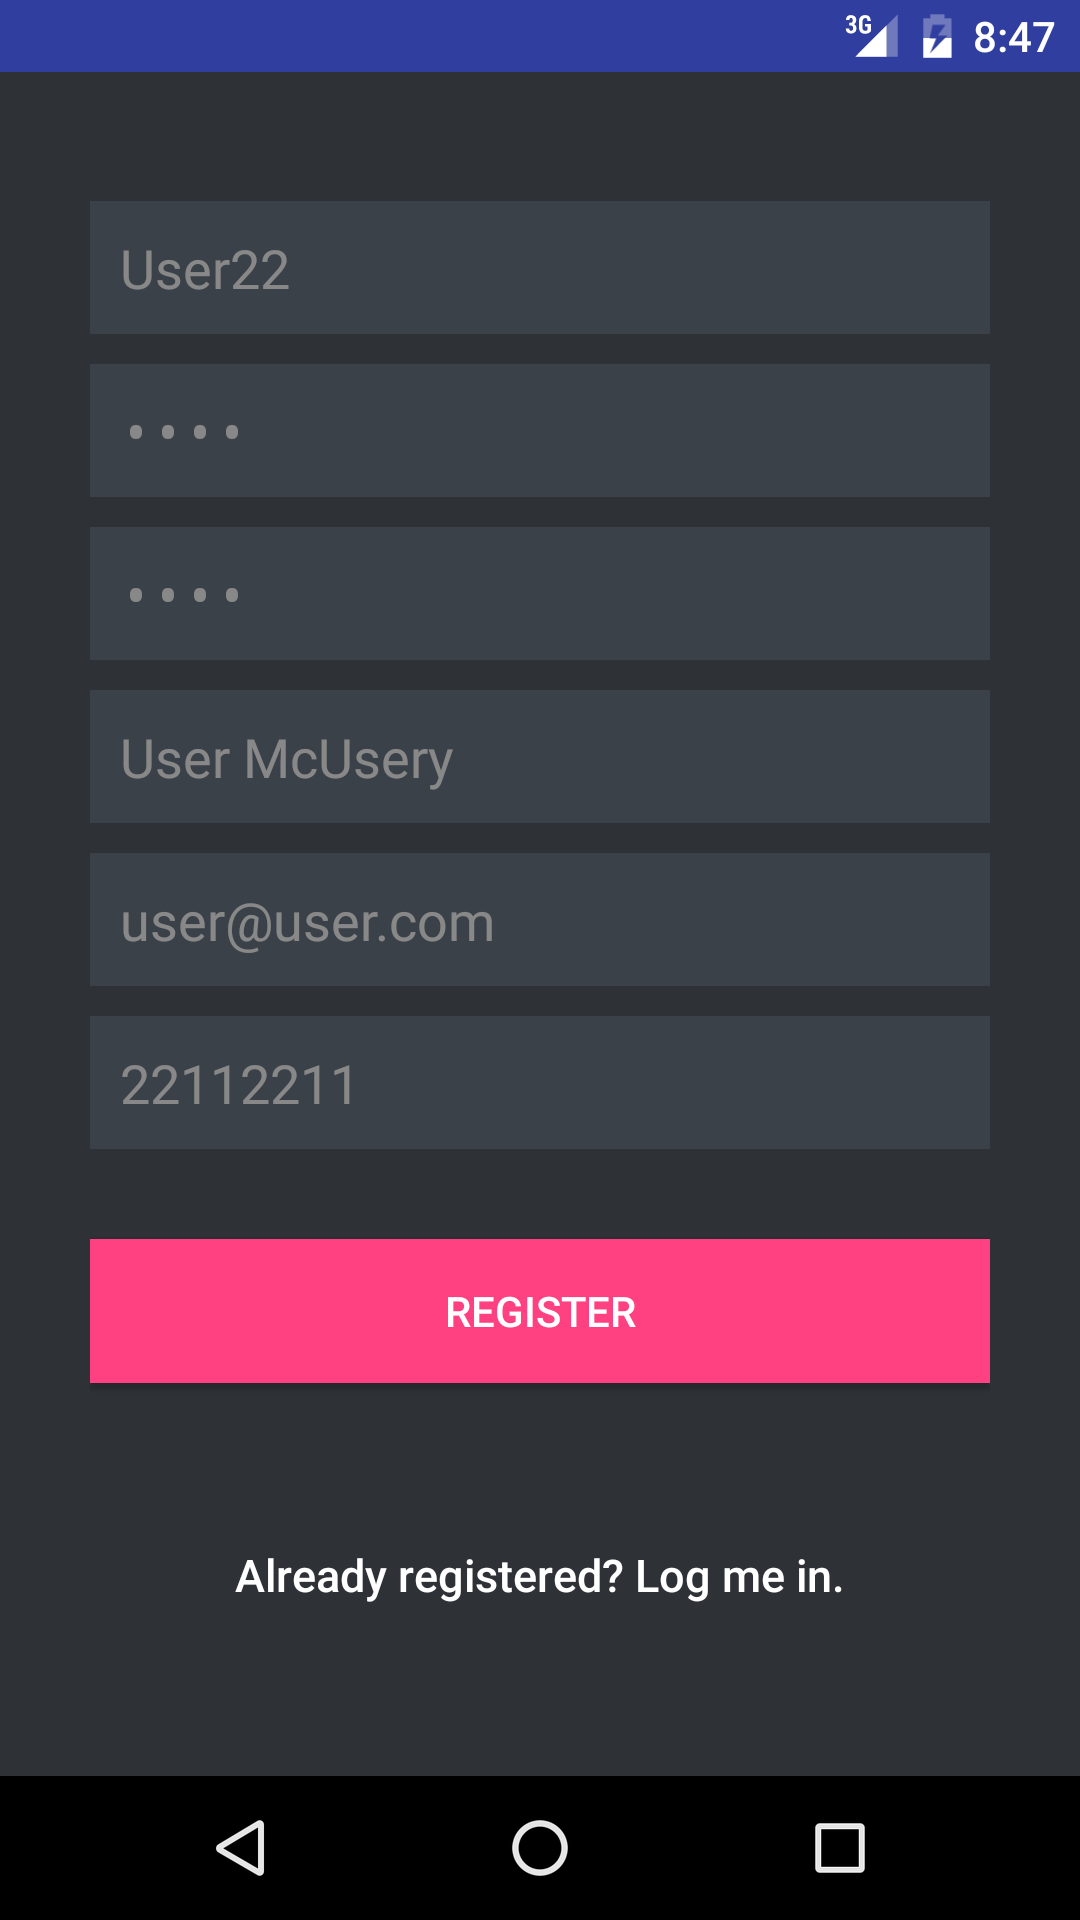
\includegraphics[width=\textwidth]{figures/s4test/newuser.png}
        \caption{Registering a new user.}
        \label{s4tp:newuser}
\end{subfigure}
\begin{subfigure}[b]{0.24\textwidth}
        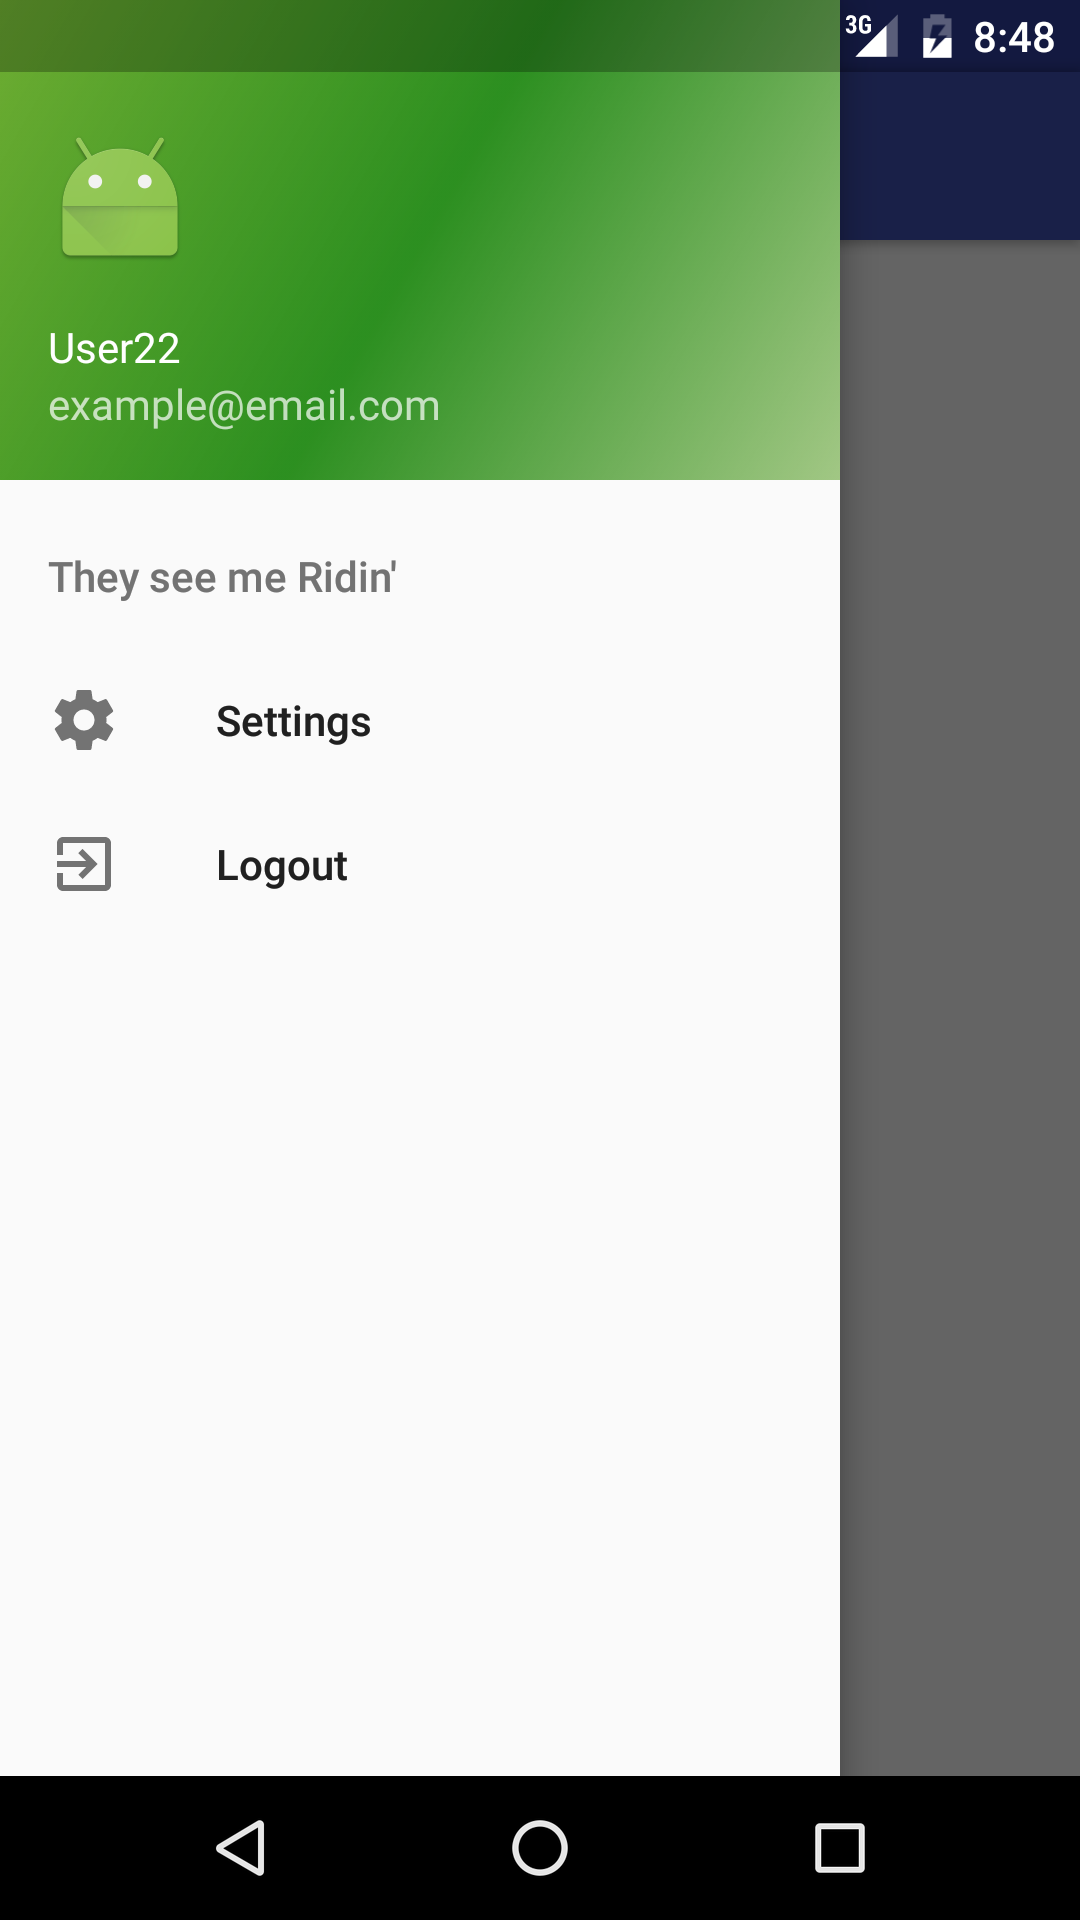
\includegraphics[width=\textwidth]{figures/s4test/newusermain.png}
        \caption{App drawer over empty mainscreen.}
        \label{s4tp:numain}
    \end{subfigure}
\begin{subfigure}[b]{0.24\textwidth}
        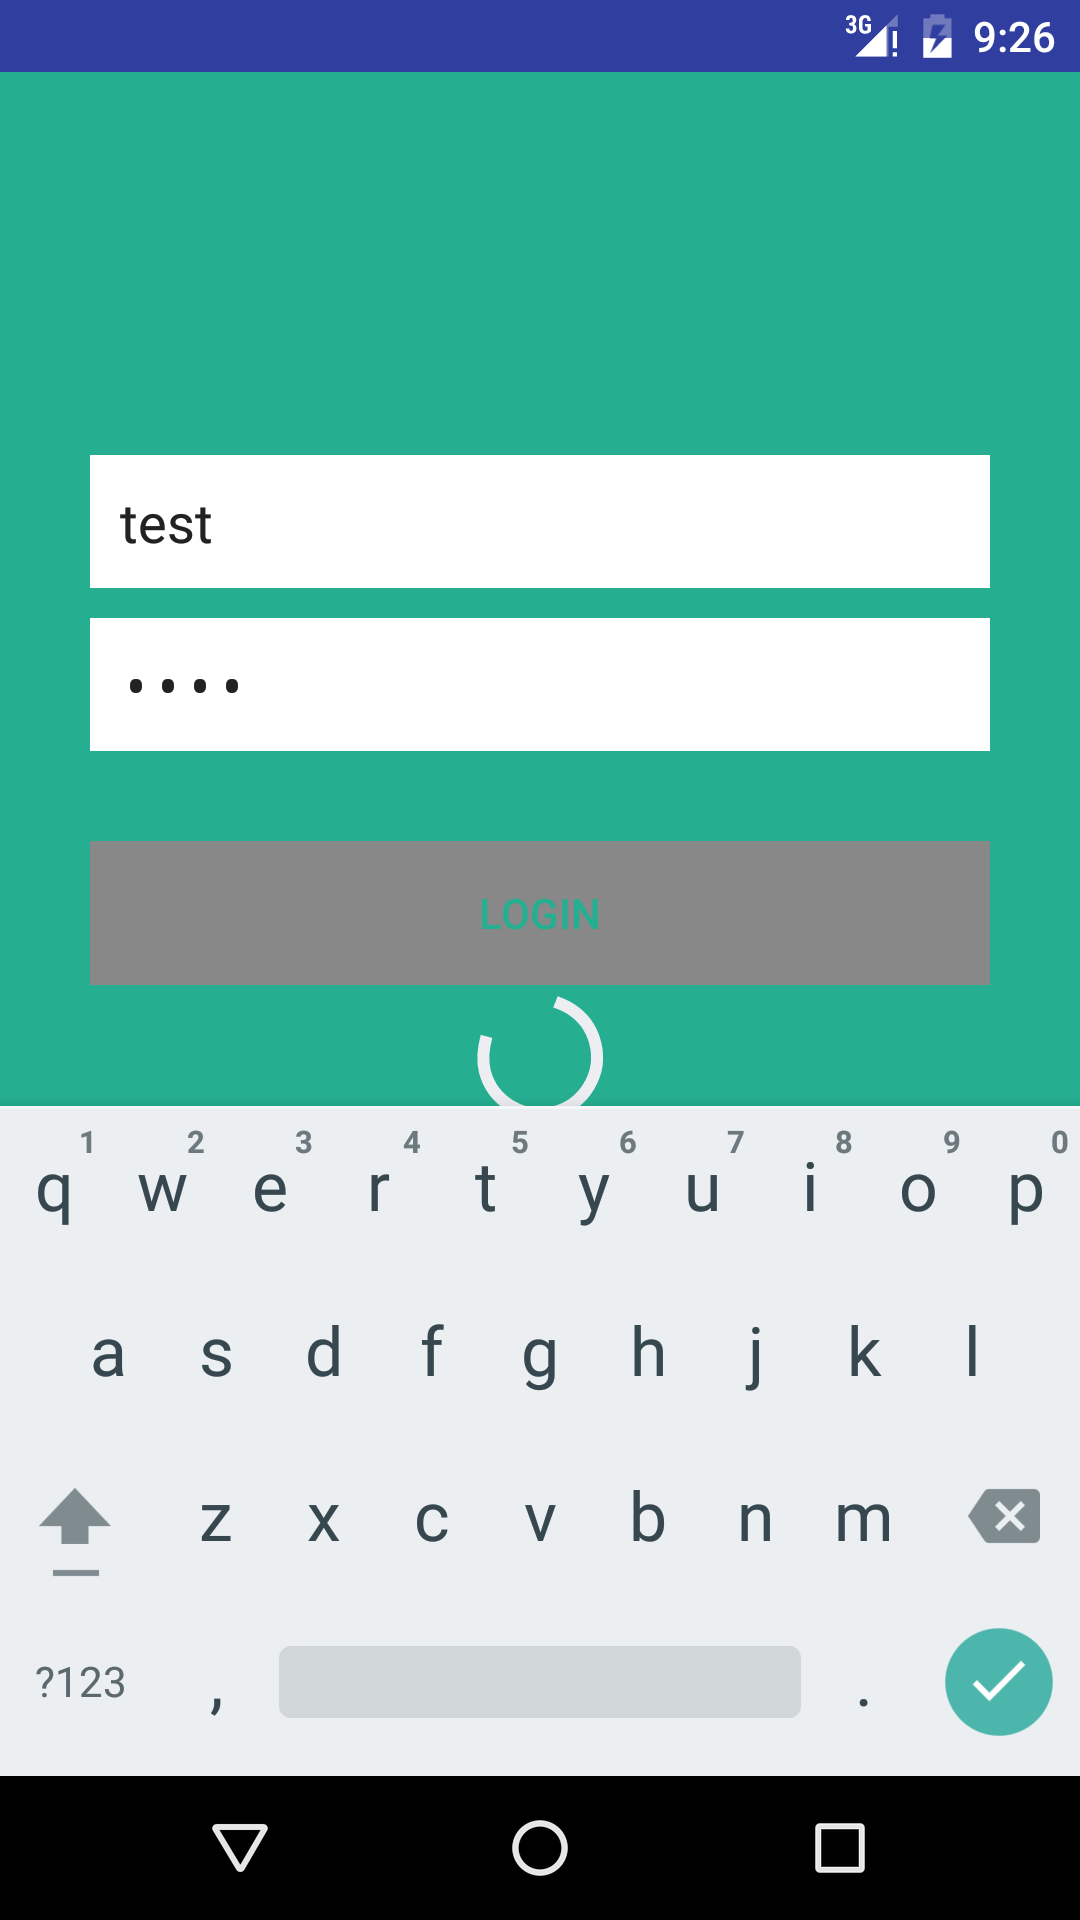
\includegraphics[width=\textwidth]{figures/s4test/logintest.png}
        \caption{Login screen for a returning user.}
        \label{s4tp:logintest}
\end{subfigure}
\begin{subfigure}[b]{0.24\textwidth}
        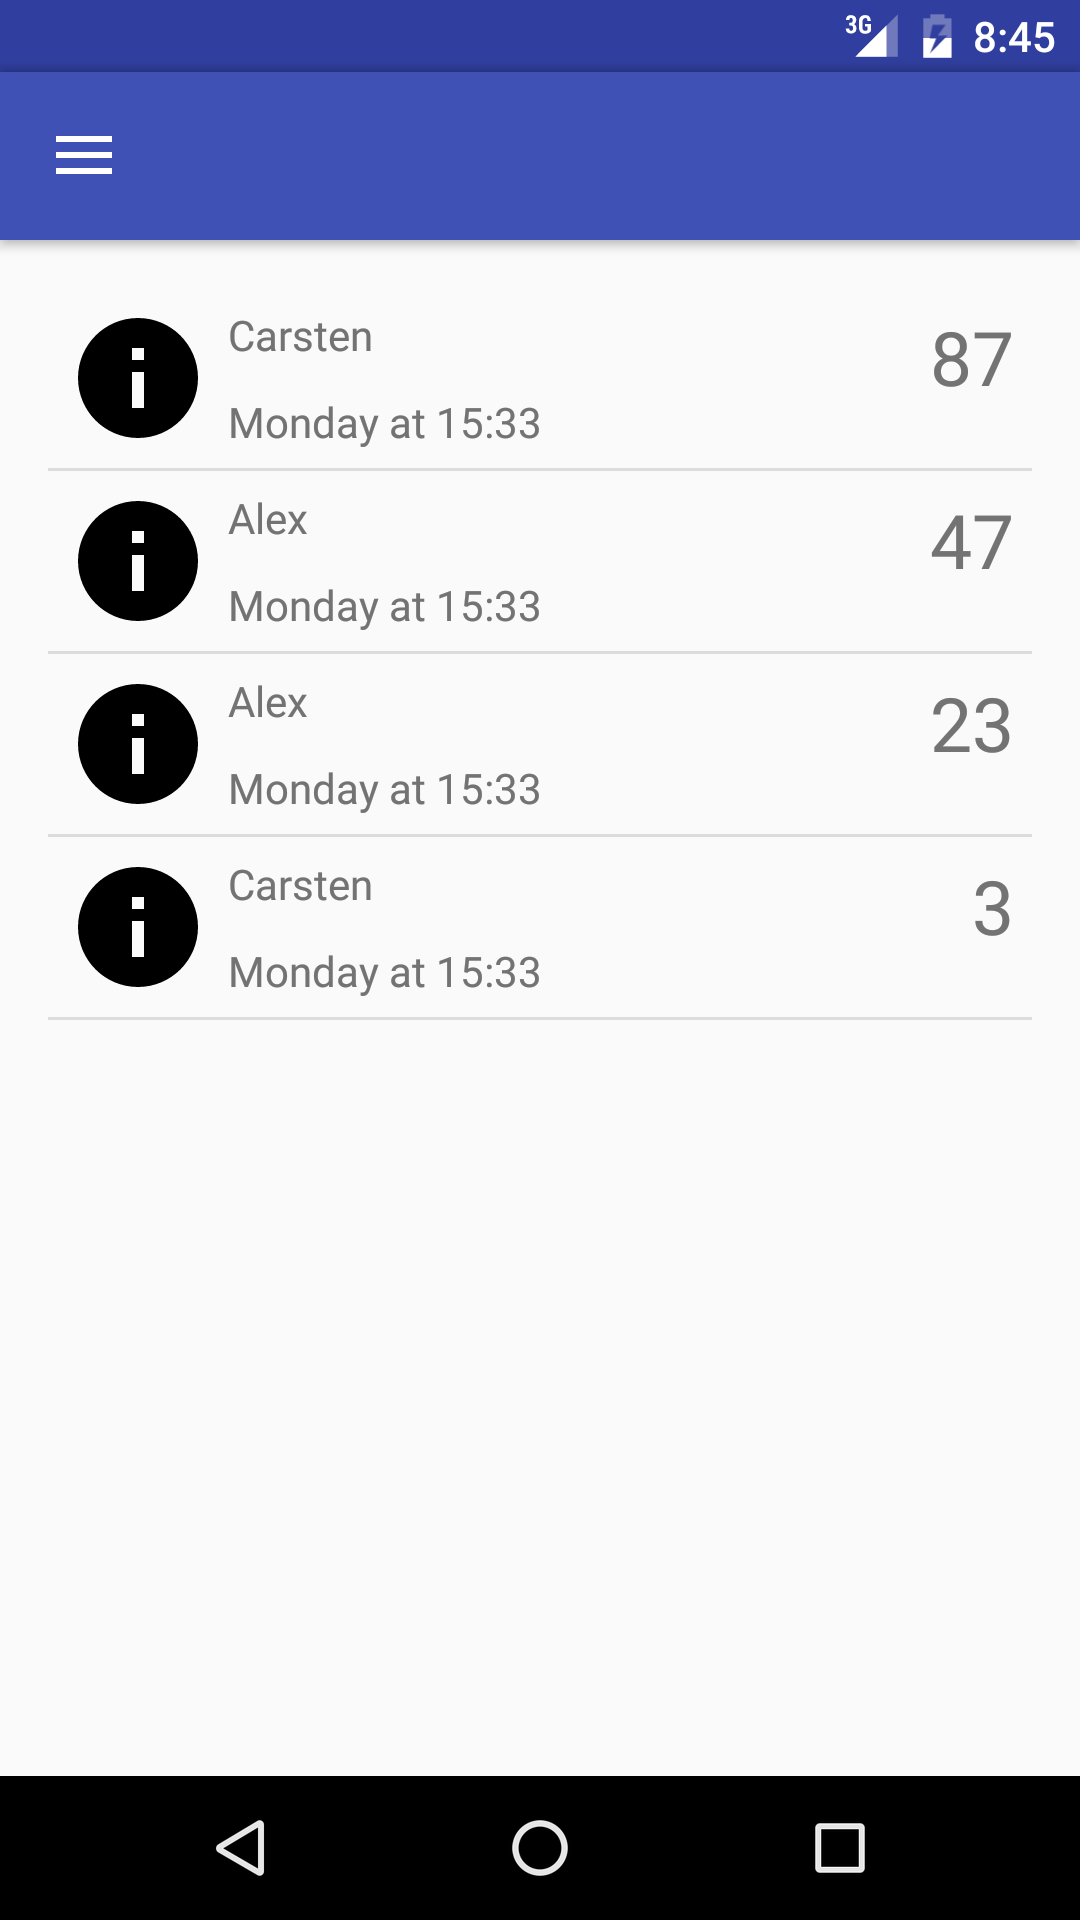
\includegraphics[width=\textwidth]{figures/s4test/testmain.png}
        \caption{Main-screen for an user with matches.}
        \label{s4tp:testmain}
\end{subfigure}
\caption{Screenshots from the acceptance test.}
\end{figure}

\subsection{Test Conclusion}
The acceptance test confirms that the developed solution fulfills the Must-have requirements.

\todo{the following is not test conclusion}
Even though every Must-have requirement is met there is still room for improvement for both  the already developed solution as well as expanding the functionality, either with additional requirements from the analysis or with new ones based on new knowledge. 
The possibilities for further development will be discussed in Section \ref{sec:future}.

%% one huge shit tack below --------------------------------------------------------------------------------------------------------------------
\iffalse
\section{Acceptance Test}
% metatext for test section
This section contains descriptions and documentation of the informal test performed on the \gls{rs} solution in the fourth sprint.
The test is the final test on the solution, and is a full system acceptance test and serves as the basis for the solution and project evaluation.
The system structure can be represented as a graph, where the app and servers are the vertices and the communication are edges. 
For a full acceptance test of the solution, each edge and vertex in the solution graph must be evaluated. 
Even though not all elements described in this section are documented in the previous implementation sections, they are considered as they are part of the solution.

% section overview
The tests yield practical implementation results, and reflect the functionality of the solution.
For the solution to pass the acceptance test it must as a minimum fulfill the Must-have requirements which were defined in Section \ref{sec:req}.
A summary list of the functional requirements can be seen below.
\begin{itemize}
	\item Graphical user interface
	\item User accounts, including login and registration
	\item Communication with the \gls{astep} system
	\item User location tracking and storage
	\item Automatically determine regular routes
	\item Automatic suggest ride sharing partners
\end{itemize}

Additionally, there are two non-functional requirements.
\begin{itemize}
	\item Development cooperation with the other \gls{astep} project groups
	\item User privacy
\end{itemize}

Some of these requirements can be fulfilled by a single part of the system while other needs two or more parts of the system to be accepted.

\subsection{\gls{rs} App}
The \gls{rs} app itself should fulfill many of the Must-have requirements.
The Must-have requirements which the app itself must satisfy are the GUI and location tracking requirements, while it is represent a part of the rest of the functional requirements and the non-functional requirement concerning privacy.

\textbf{Background location gathering}\\
The background location caching test was performed in Section \ref{subsec:bgstest2} in sprint 3, and was evaluated being fully functional, and will not be tested further here.

\textbf{Graphical User Interface}
The app implements an graphical user interface which allows access for the other functionality described in the requirements and is thereby considered fulfilled.
The GUI also supports the fulfillment of some of the other requirements, by supporting this functionality though the GUI of the app.
These are the requirements regarding the user account functionality and suggesting ridesharing partners.

\subsection{\gls{astep}}
Our contribution to the \gls{astep} system was the matching algorithm pseudo code, and a modified version of this which detects routes on the server as regular routes.
The matching algorithm was tested in sprint 3 and evaluated as sufficient for the solution a the current state, although missing a more comprehensive test with actual user routes.
The test performed in sprint 3 of the \gls{astep} route system also verified the requirement of automatically determine regular routes and therefore these two requirements pertaining to \gls{astep} are also considered completed.

\subsection{\gls{rs} Server}
Our own server have two main functions, fetching matches and allowing us to store additional user data.

\textbf{Math Storage}\\
The fetching and storage works as intended on the server. 

\textbf{User Data}\\
works quite well, preferably.

\textbf{another tested category}\\
assumed working!


\subsection{App - \gls{astep} Communication}
\textbf{Route push}\\
Pushing routes with around 10 values is working correctly, as presented in the location gathering test in Section \ref{subsec:bgstest2}.
The \gls{astep} system is, however, limited by a 2000\todo{check} character limit for the URL length.
This limits the length of the supported routes to push to \gls{astep} to around 60\todo{check} locations in a route.

\textbf{Register new user}\\
Registering a user with English letters is tested and performs as expected.

\textbf{Login}\\
Calling the \gls{astep} API with the correct arguments yield an ok signal and a token.
The token is successfully utilized to authorize other API calls.

However, there are problems logging in with passwords and usernames containing Scandinavian letters, as can be seen in Table \ref{tab:logintest}.

This seems to be a problem with Android not incorporating the mentioned letters as standard, because the \gls{astep} website API responds positively for the tested values.
This is a usability problem with the \gls{rs} app, and could be solved by implementing the support of international letters.

\begin{table}[!ht]
	\centering
	\begin{tabular}{@{}lll@{}}
		Username & Password & Result \\
		\hline
		a & a & 200 OK\\
		ø & ø & 404 not found\\
		å & a & 404 not found\\
		b & å & 401 unauthorized\\
	\end{tabular}
	\caption{Registered users login test.}
	\label{tab:logintest}
\end{table}


\subsection{RideShare Server - aSTEP Communication}
The action performed between the \gls{rs} server and \gls{astep} is to receive route matches.
It works as intended.


\subsection{App - \gls{rs} Server Communication}
\textbf{Get matches}\\
The \gls{rs} app receives matches goodly.

\textbf{Store extra data to new user}\\
Is working in beta as of May 16th.
\fi